\section{Question 3}

\begin{question}
    The data set \textit{teengamb} from the faraway package concerns a study of teenage gambling in Britain. Fit a regression model with the expenditure on gambling as the response and the sex, status, income, and verbal score as predictors. Present the summary of the model.
\end{question}

\begin{answer}
    The summary of the model is shown in the Figure \ref{fig:fig9}.
    \begin{figure}[H]
        \centering
        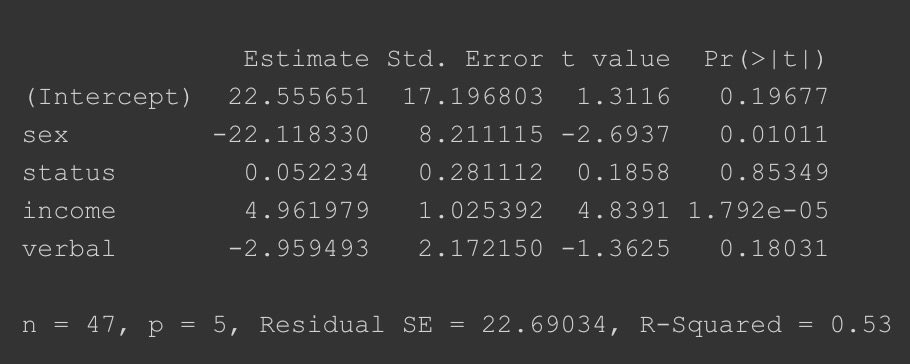
\includegraphics[width=0.7\textwidth]{Figure 9.jpeg}
        \caption{\label{fig:fig9}Summary of the model lm1}
    \end{figure}
\end{answer}

\subsection{Part a}

\begin{question}
    What proportion of variation in the response is explained by these predictors?
\end{question}

\begin{answer}
    I used the following codes finds the answer which is $r^2$ of the model. $r^2$ is computed by $\tfrac{SSR}{SST}$, where $SSR = {(\hat{y} - \overline{y})}^T - (\hat{y} - \overline{y})$, and $SST = {(y - \overline{y})}^T(y - \overline{y})$. 
    \begin{verbatim}
        # Load the data
        library(faraway)
        tg <- faraway::teengamb
        #Fit the first model
        lm1 <- lm(gamble ~ sex + status + income + verbal, data = tg)
        # Create the design matrices and hat matrices
        X <- model.matrix(lm1)
        X1 <- X[,1]
        H <- X%*%solve(t(X)%*%X)%*%t(X)
        H1 <- X1%*%solve(t(X1)%*%X1)%*%t(X1) 
        # Define y
        y = tg$gamble
        # Compute yhat
        yhat <- H%*%y 
        # Compute ybar
        ybar <- H1%*%y
        # Compute SSR and SST
        SSR <- t(yhat - ybar)%*%(yhat - ybar)
        SST <- t(y - ybar)%*%(y - ybar)
        # Compute r squared
        rsqrt <- SSR/SST
        rsqrt
    \end{verbatim}
    The result I have from the code is $r^2 = 0.5267234$. This means that $52.67234\%$ of the variation in the response variable is explained by these predictors.
\end{answer}

\subsection{Part b}

\begin{question}
    Which observation has the largest (positive) residual? Give the case number.
\end{question}

\begin{answer}
    I use the following codes to find the largest residual.
    \begin{verbatim}
        # Compute the residual
        tg$r = y - yhat
        # Find what is the maximal residual value
        rmax = max(tg$r)
        rmax
        # Find which case has largest residual
        which(tg$r == rmax)
    \end{verbatim}
    The case $24$ has the largest residual value, which is $94.25222$.
\end{answer}

\subsection{Part c}

\begin{question}
    Compute the mean and median of the residuals.
\end{question}

\begin{answer}
    \begin{verbatim}
        # Find the mean of the residuals
        mean(tg$r)
        # Find the merdian of the residuals
        median(tg$r)
    \end{verbatim}
    The codes above helped me find the mean and the median of the residuals. The mean is $-1.359206\times 10^{-14}$, and the median is $-1.451392$.
\end{answer}

\subsection{Part d}

\begin{question}
    Plot the residuals against the fitted values.
\end{question}

\begin{answer}
    I used the following codes to make the plot.
    \begin{verbatim}
        # Plot the residuals against the fitted values
        plot(lm1$fitted,tg$r,xlab = "fitted values", ylab = "residuals")
    \end{verbatim}
    The plot I got is the Figure \ref{fig:fig6}.
    \begin{figure}[H]
        \centering
        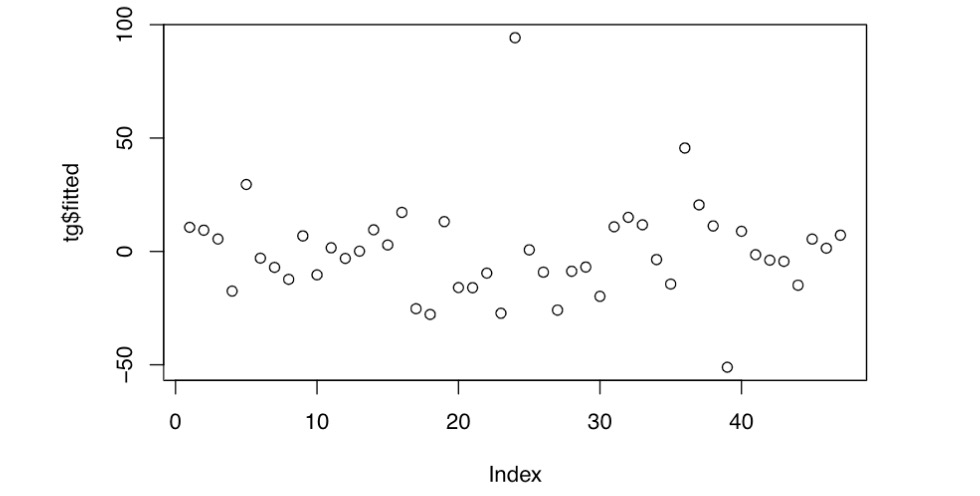
\includegraphics[width=0.7\textwidth]{Figure 6.jpeg}
        \caption{\label{fig:fig6}Plot of the residuals against the fitted values}
    \end{figure}
\end{answer}

\subsection{Part e}

\begin{question}
    Plot the residuals against the the variable income.
\end{question}

\begin{answer}
    I used the following codes to make the plot.
    \begin{verbatim}
        # Plot the residuals against the variable income
        plot(tg$income,tg$r,xlab = "income", ylab = "residuals")
    \end{verbatim}
    The plot I got is the Figure \ref{fig:fig7}.
    \begin{figure}[H]
        \centering
        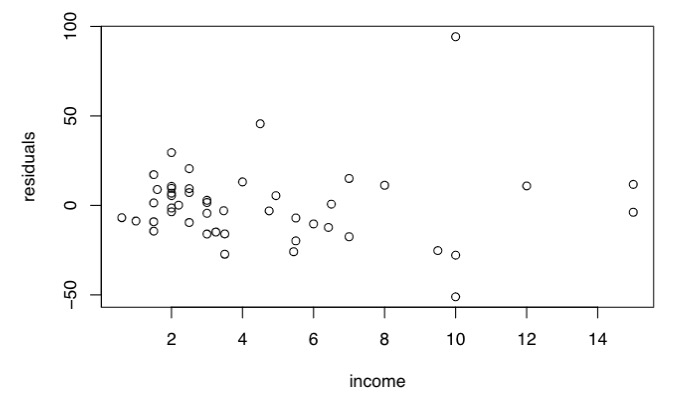
\includegraphics[width=0.7\textwidth]{Figure 7.jpeg}
        \caption{\label{fig:fig7}Plot of the residuals against the fitted values}
    \end{figure}
\end{answer}

\subsection{Part f}

\begin{question}
    For all other predictors held constant, what would be the difference (according to the model) in predicted expenditure on gambling for a male compared to a female?
\end{question}

\begin{answer}
    According to the explanation for the \textit{teengamb} data on \textit{RDocumentation} \cite{noauthor_teengamb_nodate}, for the varaible \textit{sex}, $0$ represents male, and $1$ represents female. Hence, from the fitted model in the Figure \ref{fig:fig8}, we can see that when variable \textit{sex} is $1$, the predicted expenditure on gambling is $22.11833$ lower than when \textit{sex} is $0$.
    \begin{figure}[H]
        \centering
        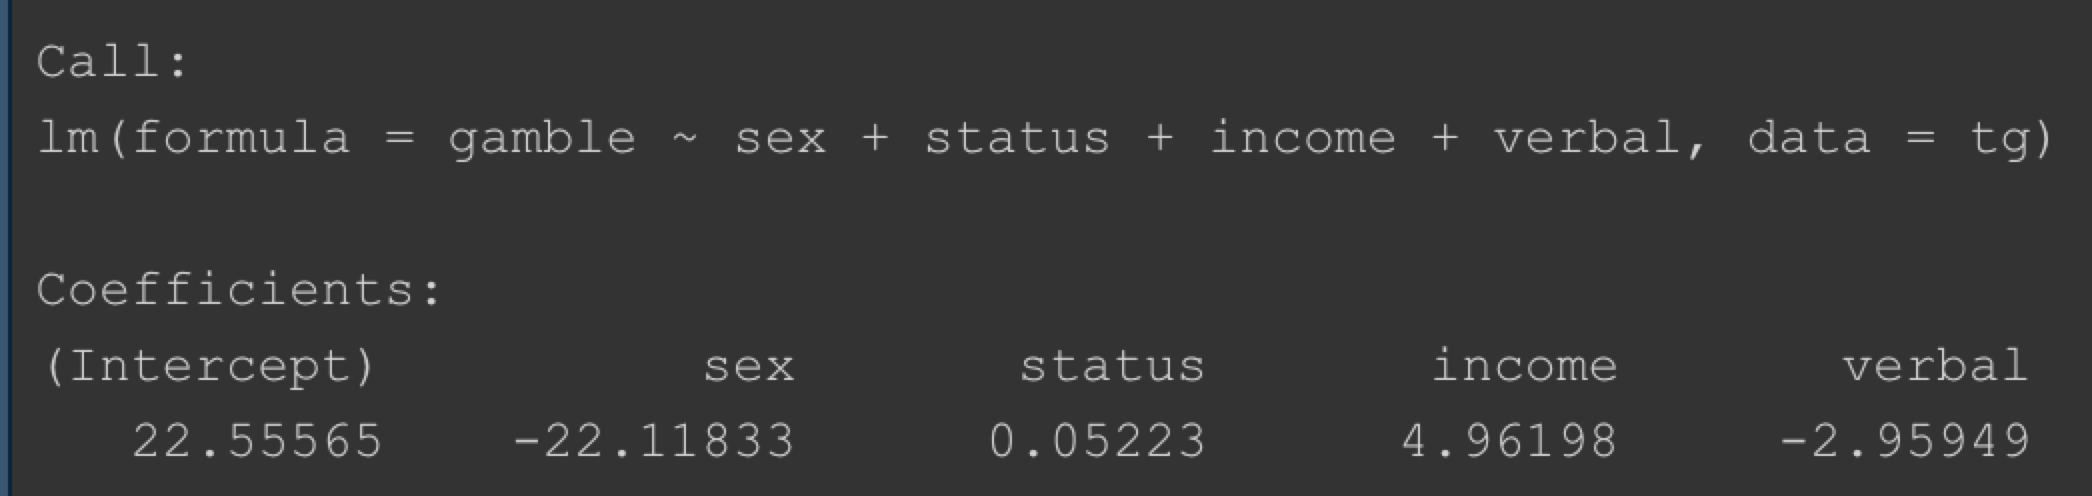
\includegraphics[width=0.7\textwidth]{Figure 8.jpeg}
        \caption{\label{fig:fig8}Model lm1}
    \end{figure}
    Thus, on average, the predicted expenditure on gambling for a male is $22.11833$ higher compared to a female.
\end{answer}
